\documentclass{article}
\usepackage{tikz}
\usetikzlibrary{shapes, positioning, fit, backgrounds, arrows.meta}
\usepackage[margin=1in]{geometry}

\begin{document}
\begin{figure}[htbp]
\centering
\vspace{1cm}
\resizebox{\textwidth}{!}{
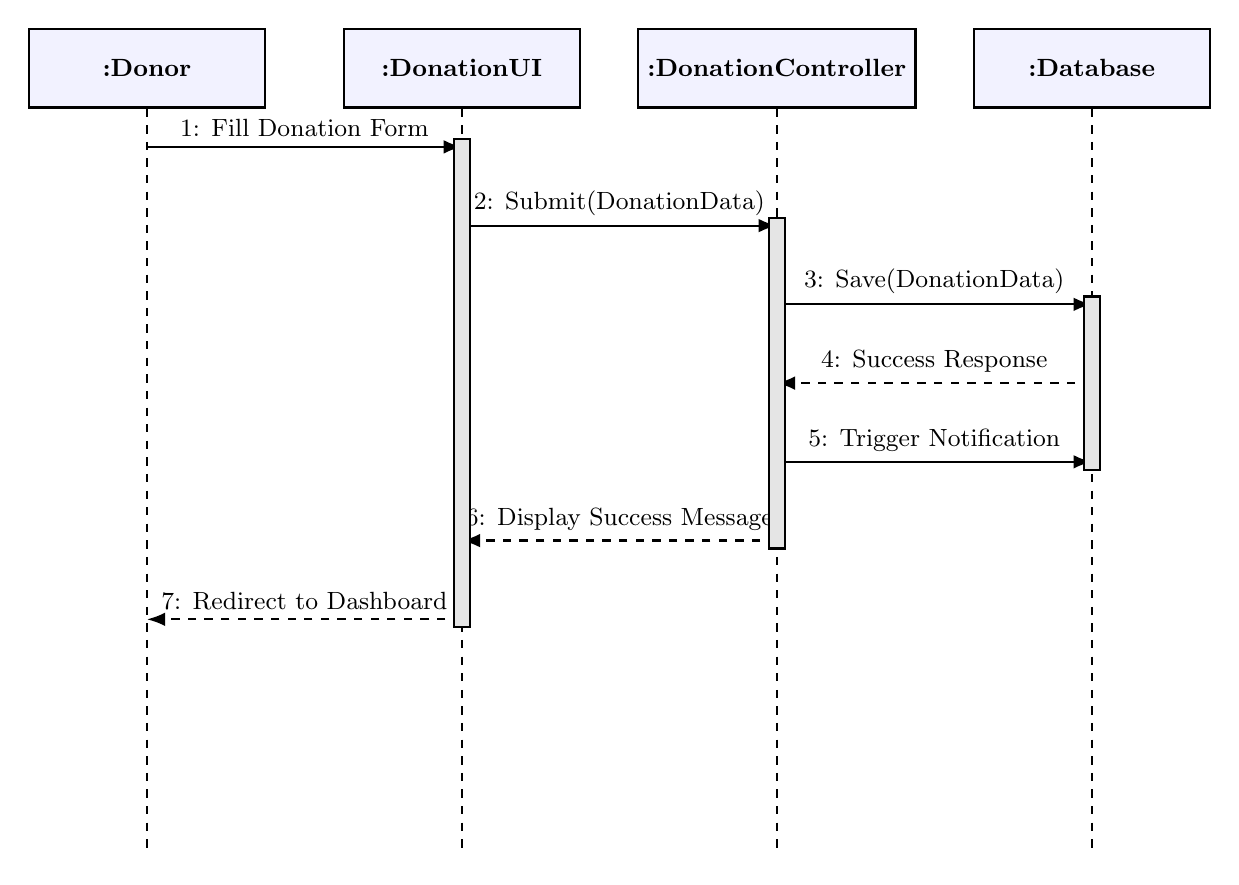
\begin{tikzpicture}[
    >=Latex, thick,
    object/.style={draw, rectangle, minimum width=3cm, minimum height=1cm, align=center, fill=blue!5, font=\small\bfseries},
    lifeline/.style={draw, dashed, thick}
]

% -------------------------
% Core Objects
% -------------------------
\node[object] (Donor) at (0, 8) {:Donor};
\node[object] (UI) at (4, 8) {:DonationUI};
\node[object] (Ctrl) at (8, 8) {:DonationController};
\node[object] (DB) at (12, 8) {:Database};

% Lifelines
\draw[lifeline] (Donor.south) -- (0, -2);
\draw[lifeline] (UI.south) -- (4, -2);
\draw[lifeline] (Ctrl.south) -- (8, -2);
\draw[lifeline] (DB.south) -- (12, -2);

% Messages
\draw[->] (0, 7) -- (4, 7) node[midway, above, font=\small] {1: Fill Donation Form};
\draw[->] (4, 6) -- (8, 6) node[midway, above, font=\small] {2: Submit(DonationData)};
\draw[->] (8, 5) -- (12, 5) node[midway, above, font=\small] {3: Save(DonationData)};

\draw[->, dashed] (12, 4) -- (8, 4) node[midway, above, font=\small] {4: Success Response};
\draw[->] (8, 3) -- (12, 3) node[midway, above, font=\small] {5: Trigger Notification};
\draw[->, dashed] (8, 2) -- (4, 2) node[midway, above, font=\small] {6: Display Success Message};
\draw[->, dashed] (4, 1) -- (0, 1) node[midway, above, font=\small] {7: Redirect to Dashboard};

% Activation Boxes (Optional visual aid)
\draw[fill=gray!20] (3.9, 7.1) rectangle (4.1, 0.9);
\draw[fill=gray!20] (7.9, 6.1) rectangle (8.1, 1.9);
\draw[fill=gray!20] (11.9, 5.1) rectangle (12.1, 2.9);

\end{tikzpicture}
}
\caption{Sequence Diagram: Donating Flow in Social Help System}
\end{figure}
\end{document}
